% questions.tex —— 1961 年·全国卷 · 题目内容片段（无答案）
% 由 tools/generate_projects.py 依来源总账自 1961/1961_数学真题_试题.md 生成，勿手改（改源 MD 后重跑）


\begin{gktip}
\textbf{题面说明}：原卷按“一（1）至（6）、二、三、四、五”编号，本文统一映射为第 1—10 题。第五部分（即第 10 题）的两个小题原卷要求选作一题；图形按原卷页面重绘为 TikZ 矢量源。
\end{gktip}

\gkpart{一、小题}

\begin{question}
\gkti{1}（1）求 $(2-x)^{10}$ 展开式里 $x^7$ 的系数。

\end{question}
\begin{question}
\gkti{2}（2）解方程：
\[
2\lg x=\lg(x+12)
\]
（注：$\lg$ 是以 10 为底的对数的符号。）

\end{question}
\begin{question}
\gkti{3}（3）求函数
\[
y=\frac{\sqrt{x-1}}{x-5}
\]
的自变量 $x$ 的允许值的范围。

\end{question}
\begin{question}
\gkti{4}（4）求
\[
\sin\frac{\pi}{12}\sin\frac{5\pi}{12}
\]
的值。

\Needspace{0.4\textheight}
\end{question}
\begin{question}
\gkti{5}（5）一个水平放着的圆柱形排水管，内半径是 $12$ 厘米。排水管的圆截面上被水淹没部分的弧含有 $150^\circ$（如图）。求这个截面上有水部分的面积。（取 $\pi=3.14$。）
\nopagebreak[4]
\begin{center}% 1961 年全国卷第 5 题：排水管圆截面中的水弓形。
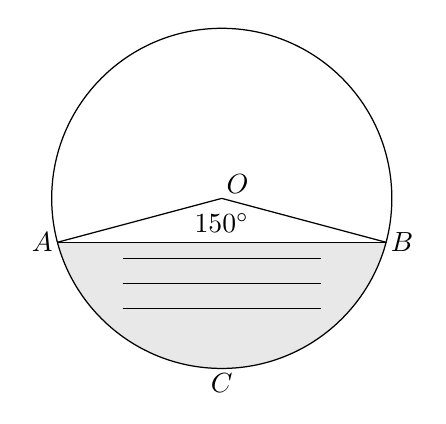
\begin{tikzpicture}[scale=0.9, line width=0.45pt,
  every node/.style={inner sep=1.5pt}]
  \coordinate (O) at (0,0);
  \coordinate (A) at (-2.32,-0.62);
  \coordinate (B) at (2.32,-0.62);
  \fill[gray!18] (A) arc (195:345:2.4) -- cycle;
  \draw (O) circle (2.4);
  \draw (A)--(B);
  \draw (O)--(A) (O)--(B);
  \foreach \y in {-1.55,-1.2,-0.85} {
    \draw (-1.4,\y)--(1.4,\y);
  }
  \node[anchor=east] at (A) {$A$};
  \node[anchor=west] at (B) {$B$};
  \node[anchor=south west] at (O) {$O$};
  \node at (0,-0.35) {$150^\circ$};
  \node[anchor=north] at (0,-2.4) {$C$};
\end{tikzpicture}
\end{center}
\nopagebreak[4]
\end{question}
\begin{question}
\gkti{6}（6）已知 $\triangle ABC$ 的一边 $BC$ 在平面 $N$ 内，$\triangle ABC$ 所在的平面与平面 $N$ 组成二面角 $\alpha$（$\alpha<90^\circ$）。从 $A$ 点作平面 $N$ 的垂线 $AA'$，$A'$ 是垂足。设 $\triangle ABC$ 的面积是 $S$，求证 $\triangle A'BC$ 的面积是 $S\cos\alpha$。

\end{question}
\gkpart{二、大题}

\begin{question}
\gkti{7}一个机器制造厂的三年生产计划，每年比上一年增产机器的台数相同。如果第三年比原计划多生产 1 千台，那么每年比上一年增长的百分数就相同，而且第三年生产的台数恰等于原计划三年生产总台数的一半。原计划每年各生产机器多少台？

\Needspace{0.4\textheight}
\end{question}
\begin{question}
\gkti{8}有一块圆环形的铁皮，它的内半径是 $45$ 厘米，外半径是 $75$ 厘米。用它的五分之一（如图中的阴影部分），作圆台形水桶的侧面。这个水桶的容积是多少立方厘米？
\nopagebreak[4]
\begin{center}% 1961 年全国卷第 8 题：圆环铁皮的五分之一扇形。
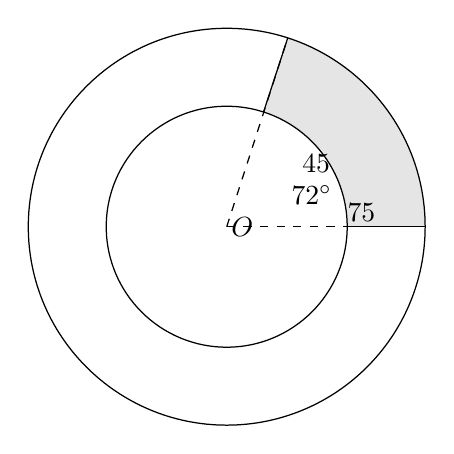
\begin{tikzpicture}[scale=0.9, line width=0.45pt,
  every node/.style={inner sep=1.5pt}]
  \coordinate (O) at (0,0);
  \fill[gray!20] (2.8,0) arc (0:72:2.8)
    -- (0.52,1.62) arc (72:0:1.7) -- cycle;
  \draw (O) circle (2.8);
  \draw (O) circle (1.7);
  \draw (2.8,0)--(1.7,0);
  \draw (0.86,2.66)--(0.52,1.62);
  \draw[dashed] (O)--(2.8,0);
  \draw[dashed] (O)--(0.86,2.66);
  \node[anchor=west] at (O) {$O$};
  \node[anchor=south] at (1.9,0) {$75$};
  \node[anchor=south west] at (1.0,0.7) {$45$};
  \node at (1.2,0.45) {$72^\circ$};
\end{tikzpicture}
\end{center}
\nopagebreak[4]
\Needspace{0.4\textheight}
\end{question}
\begin{question}
\gkti{9}在平地上有 $A$、$B$ 两点。$A$ 在山的正东。$B$ 在山的东南，且在 $A$ 的西 $65^\circ$ 南 $300$ 米的地方。在 $A$ 测得山顶的仰角是 $30^\circ$，求山高。（$\sin70^\circ=0.940$，精确到 10 米。）
\nopagebreak[4]
\begin{center}% 1961 年全国卷第 9 题：由 A、B 方位与仰角测山高。
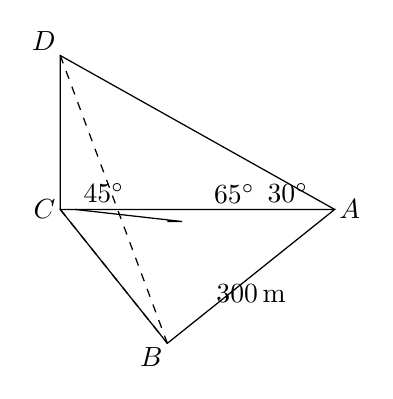
\begin{tikzpicture}[scale=0.85, line width=0.45pt,
  every node/.style={inner sep=1.5pt}]
  \coordinate (A) at (2.5,0.4);
  \coordinate (C) at (-1.6,0.4);
  \coordinate (D) at (-1.6,2.7);
  \coordinate (B) at (0.0,-1.6);
  \draw (A)--(B)--(C)--cycle;
  \draw (C)--(D)--(A);
  \draw[dashed] (C)--(B);
  \draw[dashed] (D)--(B);
  \draw (C)+(0.22,0)--(0.22,0.22)--(0,0.22);
  \node[anchor=west] at (A) {$A$};
  \node[anchor=north east] at (B) {$B$};
  \node[anchor=east] at (C) {$C$};
  \node[anchor=south east] at (D) {$D$};
  \node at (1.8,0.65) {$30^\circ$};
  \node at (1.0,0.63) {$65^\circ$};
  \node at (-0.95,0.65) {$45^\circ$};
  \node[anchor=north] at (1.25,-0.65) {$300\,\mathrm m$};
\end{tikzpicture}
\end{center}
\nopagebreak[4]
\end{question}
\begin{question}
\gkti{10}下面甲、乙两题，选作一题。

甲、$k$ 是什么实数的时候，方程
\[
x^2-2(k+3)x+3k^2+1=0
\]
有实数根？

乙、设方程
\[
8x^2-(8\sin\alpha)x+2+\cos2\alpha=0
\]
的两个根相等，求 $\alpha$。

\end{question}